\documentclass[beamer]{standalone}
\usepackage{circuitikz}

\tikzstyle{block} = [draw, fill=blue!20, rectangle, 
    minimum height=3em, minimum width=6em]
\tikzstyle{sum} = [draw, fill=blue!20, circle, node distance=1cm]
\tikzstyle{input} = [coordinate]
\tikzstyle{output} = [coordinate]
\tikzstyle{pinstyle} = [pin edge={to-,thin,black}]

\begin{document}

\title[Electronics 1]{Introduction to Digital Circuits}

\begin{frame} 
  \titlepage
\end{frame}

\begin{frame}{Final Lab and Final Exam}
\begin{block}{Final lab}
\begin{itemize}
\item Last week of labs, April 28-29-30
\item Assigned random groups of two students
\item You will do the design and build the circuit together, taking notes in a blue book
\item Each person individually will have to explain and answer some questions about the circuit
\end{itemize}
\end{block}
\begin{block}{Final exam}
\begin{itemize}
\item May 4, 9am--noon
\item Similar setup as midterm
\end{itemize}
\end{block}
\centerline{Best score of final lab and final exam will count as ``final exam'' grade.}
\end{frame}

\begin{frame}{Midterm Test}
\begin{block}{What about the midterm?}
\begin{itemize}
\item You will receive the midterm back in lab next week
\item You can correct your answers and hand them in during your final lab for 50\% credit
\end{itemize}
\end{block}
\end{frame}

\begin{frame}{Digital Circuits}
\begin{block}{Definition of ``digital''}
The signal can only have two levels: yes/no, on/off, 1/0
\end{block}
\begin{block}{Electronic implementation}
In real electronic circuits we will consider high/low voltage levels:
\begin{itemize}
\item high = 1 (e.g. +3.3\,V in CMOS logic, +5\,V in TTL logic, or -0.8\,V in NIM logic)
\item low = 0 (ground, but in practice implemented as a range)
\end{itemize}
\end{block}
\begin{block}{Thresholds}
\begin{itemize}
\item $V_{OH}$: Minimum OUTPUT Voltage level a device will provide for a HIGH signal.
\item $V_{IH}$: Minimum INPUT Voltage level to be considered HIGH.
\item $V_{OL}$: Maximum OUTPUT Voltage level a device will provide for a LOW signal.
\item $V_{IL}$: Maximum INPUT Voltage level to be considered LOW.
\end{itemize}
\end{block}
\end{frame}

\begin{frame}{Logic Levels}
\begin{center}
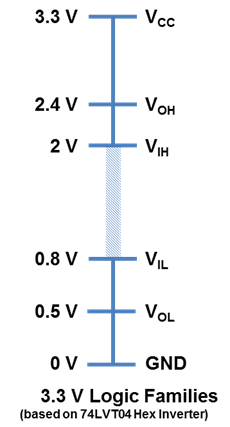
\includegraphics[width=0.26\textwidth]{pics/CMOS_levels}
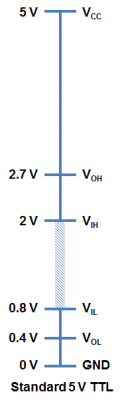
\includegraphics[width=0.21\textwidth]{pics/TTL_levels}
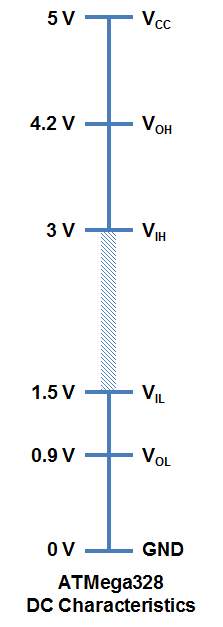
\includegraphics[width=0.25\textwidth]{pics/arduino_levels}
\end{center}
\end{frame}

\begin{frame}{Truth Tables}
\begin{block}{Definition}
Explicit listing of output state for all possible input states
\end{block}
\begin{center}
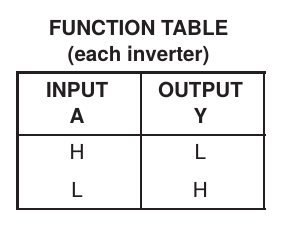
\includegraphics[width=0.3\textwidth]{pics/NOR_truth_table}
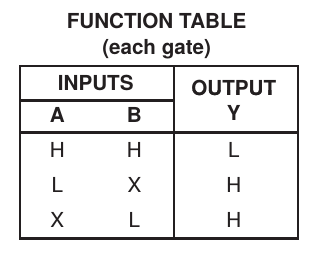
\includegraphics[width=0.3\textwidth]{pics/NAND_truth_table}
\end{center}
Note: `X' signifies any input.
\end{frame}

\begin{frame}{Common Logic Gates}
\begin{itemize}
\item NOT: $OUT = \bar{A}_{in}$ \\
\centerline{\begin{circuitikz} \draw (0,0) node[not port]{}; \end{circuitikz}}
\item OR: $OUT = A_{in} + B_{in}$ \\
\centerline{\begin{circuitikz} \draw (0,0) node[or port]{}; \end{circuitikz}}
\item AND: $OUT = A_{in} \cdot B_{in}$ \\
\centerline{\begin{circuitikz} \draw (0,0) node[and port]{}; \end{circuitikz}}
\item NAND: $OUT = \bar{A_{in} \cdot B_{in}}$ (universal NAND, NOR logic) \\
\centerline{\begin{circuitikz} \draw (0,0) node[nand port]{}; \end{circuitikz}}
\item XOR: $OUT = A_{in} \oplus B_{in}$ \\
\centerline{\begin{circuitikz} \draw (0,0) node[xor port]{}; \end{circuitikz}}
\end{itemize}
\end{frame}

\begin{frame}{Bit Adder}
\begin{block}{Construct the logic for an adder of 2 bits}
\begin{itemize}
\item Input is two single bits $A$ and $B$, output is a 2-bit binary number
\item What is the truth table for the two output bits $OUT_1$ and $OUT_2$?
\end{itemize}
\end{block}
\begin{block}<2>{Solution}
\begin{itemize}
\item $OUT_1 = A \cdot B$
\item $OUT_2 = A \oplus B$
\end{itemize}
\end{block}
\end{frame}

\begin{frame}{Universal NOR}
\begin{block}{Construct an NOT gate with just a NOR}
\end{block}
\begin{block}<2>{Solution}
\begin{circuitikz}
\draw (0,0) node[nor port](nor){};
\draw (nor.out) to[short,-o] ++(0.5,0) node[right]{$OUT$};
\draw (nor.in 1) -| (-2,0);
\draw (nor.in 2) -| (-2,0);
\draw (-2,0) to[short,-o] ++(-0.5,0) node[left]{$IN$};
\end{circuitikz}
\end{block}
\end{frame}

\end{document}
